\documentclass{beamer}

\beamertemplatenavigationsymbolsempty
\setbeamertemplate{footline}[frame number]

\usepackage{tikz}
\usetikzlibrary{matrix,positioning,arrows.meta,arrows,calc}

\title[Crisis]
{Decentralised location verification system}
\author{Conor Taylor}
\date{
	B.A.(Mod.) Computer Science\\
	Final Year Project, April 2016\\
	Supervisor: Stephen Barrett
}

\begin{document}

	\frame{\titlepage}
	
	\begin{frame}
    	\frametitle{Problem}
    	A system that allows participants to verify a users claimed location.
    	\\
    	\null
    	\visible<2->{
    		Goals:
   			\begin{itemize}
    			\item<3-> False location claims must be detectable.
    			\item<4-> Privacy protecting.
    			\item<5-> Cannot rely on any centralised resources.
    			\item<6-> Capable of running in the background on mobile devices.
    		\end{itemize}
    	}
	\end{frame}
	
	\begin{frame}
		\frametitle{Background}
		There are \textbf{no} known existing decentralised location proof systems.
		\\
		\null
		Existing centralised solutions: hardware and/or software
	\end{frame}
	
	\begin{frame}
		\frametitle{Design}
		3 distinct entities:
		\begin{itemize}
			\item Mobile node $\vcenter{\hbox{
\includegraphics[scale=0.2]{diagrams/overview-presentation/mobile-node.png}}}$
			\item Miner node $\vcenter{\hbox{
\includegraphics[scale=0.2]{diagrams/overview-presentation/miner-node.png}}}$
			\item Verifier node $\vcenter{\hbox{
\includegraphics[scale=0.2]{diagrams/overview-presentation/verifier-node.png}}}$
		\end{itemize}
	\end{frame}
	
	\begin{frame}
		\frametitle{Design}
		\framesubtitle{Overview}
		\begin{figure}[H]
			\begin{center}
				\resizebox {\columnwidth} {!} {
					\includegraphics<1>{diagrams/overview-presentation/Overview-13.png}
					\includegraphics<2>{diagrams/overview-presentation/Overview-12.png}
					\includegraphics<3>{diagrams/overview-presentation/Overview-11.png}
					\includegraphics<4>{diagrams/overview-presentation/Overview-10.png}
					\includegraphics<5>{diagrams/overview-presentation/Overview-9.png}
					\includegraphics<6>{diagrams/overview-presentation/Overview-8.png}
					\includegraphics<7>{diagrams/overview-presentation/Overview-7.png}
					\includegraphics<8>{diagrams/overview-presentation/Overview-6.png}
					\includegraphics<9>{diagrams/overview-presentation/Overview-5.png}
					\includegraphics<10>{diagrams/overview-presentation/Overview-4.png}
					\includegraphics<11>{diagrams/overview-presentation/Overview-3.png}
					\includegraphics<12>{diagrams/overview-presentation/Overview-2.png}
					\includegraphics<13>{diagrams/overview-presentation/Overview-1.png}
					\includegraphics<14>{diagrams/overview-presentation/Overview-0.png}
			}
			\end{center}
		\end{figure}
	\end{frame}
	
	\begin{frame}
		\frametitle{Design}
		\framesubtitle{Identities}
		Used to anonymously identify a node in a transaction.
		\newline
		
		Balancing goals:
		\begin{itemize}
			\item False location claims must be detectable.
			\item Privacy protecting.
		\end{itemize}
	\end{frame}
	
	\begin{frame}
		\frametitle{Design}
		\framesubtitle{Identities: Nonce Lists}
		\begin{figure}[H]
			\resizebox {\columnwidth} {!} {\begin{tikzpicture}[>=latex]

\tikzset{
mymat/.style={
  matrix of math nodes,
  text height=2.5ex,
  text depth=0.75ex,
  text width=5.25ex,
  align=center,
  column sep=-\pgflinewidth
  },
mymats/.style={
  mymat,
  text width=8ex,
  nodes={draw}
  }  
}

\matrix[mymat,anchor=west,row 1/.style={nodes=draw}]
at (0,0) 
(mat1)
{
\only<1>{4827 & 1928 & 9183}
\only<2->{4827 & 1928 & 9183 & 0047}\\
};
\matrix[mymats=white,anchor=west]
at (0,-3) 
(mat3)
{
\only<-2>{12ef5a1 & c100e9d & 038ef6b}
\only<3->{12ef5a1 & c100e9d & 038ef6b & ee3bc14} \\
};

\node[left=0pt of mat1]
  (cella) {Nonce list:};
  
\node[left=0pt of mat3]
  (cella) {Identities:};
  
\only<3->{ 
\node (key) at ($(mat1-1-4.south)!0.5!(mat3-1-4.north)$) {$K^+(0047)$};
}

\begin{scope}[shorten <= -2pt]
\draw[*->]
  (mat1-1-1.south) -- (mat3-1-1.north);
\draw[*->]
  (mat1-1-2.south) -- (mat3-1-2.north);
\draw[*->]
  (mat1-1-3.south) -- (mat3-1-3.north);
\only<3->{
\draw[*-]
  (mat1-1-4.south) -- (key);
}
\only<3->{
\draw[->]
  (key) -- (mat3-1-4.north);
}
\end{scope}
\end{tikzpicture}}
		\end{figure}
	\end{frame}
	
	\begin{frame}
		\frametitle{Design}
		\framesubtitle{Identities: Duplication}
		Identity duplication is unavoidable in a decentralised system.
		\visible<2->{
		\begin{table}[]
			\begin{tabular}{l|l}
				\textbf{ID} & \textbf{Contents}\\\hline
				\dots & \\\hline
				ffa0 & \\\hline
				ffa1 & \\\hline
				ffa2 & $T_{A4}$ \visible<3->{, \textcolor{red}{$T_{C102}$}}\\\hline
				ffa3 & \\\hline
				ffa4 & $T_{B87}$\\\hline
				\dots & \\
			\end{tabular}
		\end{table}
		}
	\end{frame}
	
	\begin{frame}
		\frametitle{Design}
		\framesubtitle{Transactions}
		Transactions are created when two mobile nodes physically meet.
		\begin{itemize}
			\item Ad-hoc bluetooth connection between the nodes.
		\end{itemize}		
		
		\begin{center}
			\resizebox {0.35\columnwidth} {!} {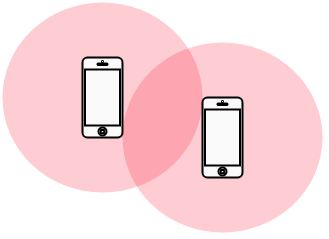
\includegraphics{diagrams/overview-presentation/mobile-node-meet.png}}
		\end{center}
	\end{frame}
	
	\begin{frame}
		\frametitle{Design}
		\framesubtitle{Transactions II}
		\begin{figure}[t]
			\resizebox {\columnwidth} {!} {\begin{tikzpicture}

\node[draw] (A) at (0,0) {\textbf{Node A}};
\only<2>{\node[above= 0mm of A] {\textcolor{red}{$n$}};}
\only<3->{\node[above= 0mm of A] {$n$};}

\only<3> {\node[below left= 0mm of A] (k_a) {\textcolor{red}{$K^+_A$, $K^-_A$}};}
\only<4-> {\node[below left= 0mm of A] (k_a) {$K^+_A$, $K^-_A$};}

\only<4> {\node[below= 0mm of k_a] (nl_a) {\textcolor{red}{$NL_A$}};}
\only<5-> {\node[below= 0mm of k_a] (nl_a) {$NL_A$};}
	
\only<5> {\node[below right=0mm and -1cm of nl_a] (id_a) {\textcolor{red}{$ID_{An} = K^+_A(NL_A[n])$}};}
\only<6-> {\node[below= 0mm of nl_a] (id_a) {$ID_{An}$};}

\only<6> {\node[below= 0mm of id_a] (ts_a) {\textcolor{red}{$ts_A$}};}
\only<7-> {\node[below= 0mm of id_a] (ts_a) {$ts_A$};}

\only<7> {\node[below= 0mm of ts_a] (loc_a) {\textcolor{red}{$loc_{A}$}};}
\only<8-> {\node[below= 0mm of ts_a] (loc_a) {$loc_{A}$};}

\only<15>{
\node[below= 0mm of loc_a] (id_b_a) {\textcolor{red}{$ID_{Bm}$}};
\node[below= 0mm of id_b_a] (ts_b_a) {\textcolor{red}{$ts_B$}};
\node[below= 0mm of ts_b_a] (loc_b_a) {\textcolor{red}{$loc_{B}$}};
}
\only<16->{
\node[below= 0mm of loc_a] (id_b_a) {$ID_{Bm}$};
\node[below= 0mm of id_b_a] (ts_b_a) {$ts_B$};
\node[below= 0mm of ts_b_a] (loc_b_a) {$loc_{B}$};
}


\node[draw] (B) at (5,0) {\textbf{Node B}};
\only<2>{\node[above= 0mm of B] {\textcolor{red}{$m$}};}
\only<3->{\node[above= 0mm of B] {$m$};}

\only<8->{
\node[below right= 0mm of B] (k_b) {$K^+_B$, $K^-_B$};
\node[below= 0mm of k_b] (nl_b) {$NL_B$};
\node[below= 0mm of nl_b] (id_b) {$ID_{Bm}$};
\node[below= 0mm of id_b] (ts_b) {$ts_B$};
\node[below= 0mm of ts_b] (loc_b) {$loc_{B}$};
}

\only<11>{
\node[below= 0mm of loc_b] (id_a_b) {\textcolor{red}{$ID_{An}$}};
\node[below= 0mm of id_a_b] (ts_a_b) {\textcolor{red}{$ts_A$}};
\node[below= 0mm of ts_a_b] (loc_a_b) {\textcolor{red}{$loc_{A}$}};
}
\only<12->{
\node[below= 0mm of loc_b] (id_a_b) {$ID_{An}$};
\node[below= 0mm of id_a_b] (ts_a_b) {$ts_A$};
\node[below= 0mm of ts_a_b] (loc_a_b) {$loc_{A}$};
}

\only<9>{
\draw[->] (A) -- (B) node[midway,below] (treq_label)
	{\textcolor{red}{$T_{req}$}};
}
\only<10>{
\draw[->] (A) -- (B) node[midway,below] (treq_label)
	{$T_{req}$};
}
\only<10>{
\node[below= 0mm of treq_label] {\textcolor{red}{$ID_{An} | ts_A | loc_A$}};
}

\only<12>{
\node[left= 5mm of loc_b] (v_b) {\small{\textit{\textcolor{red}{verify $|ts_A-ts_B| < \epsilon_{ts}$}}}};
\node[below= -2mm of v_b] {\small{\textit{\textcolor{red}{$\&\& |loc_A-loc_B| < \epsilon_{loc}$}}}};
}

\only<13>{
\draw[->] (B) -- (A) node[midway,below] (tres_label)
	{\textcolor{red}{$T_{res}$}};
}
\only<14>{
\draw[->] (B) -- (A) node[midway,below] (tres_label)
	{$T_{res}$};
}
\only<14>{
\node[below= 0mm of tres_label] {\textcolor{red}{$ID_{Bm} | ts_B | loc_B$}};
}

\only<16>{
\node[right= 5mm of loc_a] (v_a) {\small{\textit{\textcolor{red}{verify $|ts_A-ts_B| < \epsilon_{ts}$}}}};
\node[below= -2mm of v_a] {\small{\textit{\textcolor{red}{$\&\& |loc_A-loc_B| < \epsilon_{loc}$}}}};
}

\end{tikzpicture}}
		\end{figure}
	\end{frame}
\end{document}